\RequirePackage{fix-cm}  % Korrektur für CM-Schriftgrößen
\documentclass[a4paper,12pt]{report}

% ========================
%  KODIERUNG & SCHRIFTARTEN
% ========================
\usepackage[T1]{fontenc}        % T1-Schriftkodierung
\usepackage[utf8]{inputenc}     % UTF8-Eingabekodierung
\usepackage{lmodern}
\usepackage{helvet}             % Arial-Schriftart
\renewcommand{\familydefault}{\sfdefault}  % Sans-Serif als Standard
\usepackage{mathpazo}           % Palatino für Matheumgebungen
\usepackage[italic]{mathastext} % Helvetica in Matheumgebungen
\usepackage{textcomp}           % Zusätzliche Textzeichen

% ========================
%  SPRACHE & ZITIERSTIL
% ========================
\usepackage[ngerman]{babel}     % Deutsche Silbentrennung
\usepackage[style=chem-angew]{biblatex}  % Chemie-Zitierstil
\addbibresource{1.bib}          % Literaturdatenbank

% ========================
%  SEITENLAYOUT
% ========================
\usepackage[top=2cm, bottom=3cm, left=2cm, right=2cm]{geometry}
\usepackage{setspace}           % Zeilenabstand
\onehalfspacing                 % 1.5-facher Zeilenabstand
\usepackage{parskip}            % Absatzabstände
\setlength{\parindent}{0mm}     % Keine Einrückung
\usepackage{fancyhdr}           % Kopf- und Fußzeilen
\usepackage{pdflscape}          % Querformat-Seiten

% ========================
%  MATHEMATIK & CHEMIE
% ========================
\usepackage{amsmath, amssymb, mathtools}  % Mathepakete
\usepackage{chemformula}        % Chemische Formeln
\usepackage[version=4]{mhchem}  % Erweiterte Chemienotation
\usepackage{textgreek}          % Griechische Buchstaben im Text

% ========================
%  EINHEITEN & MESSWERTE
% ========================
\usepackage{siunitx}            % SI-Einheiten und wissenschaftliche Notation
\sisetup{
  detect-all,                   % Automatische Schriftarterkennung
  range-units = single          % Einheitenbereichsdarstellung
}
\DeclareSIUnit\angstrom{\text{Å}}  % Ångström-Definition

% ========================
%  TABELLEN & ABBILDUNGEN
% ========================
\usepackage{tabularx}           % Flexible Tabellen
\usepackage{tabularray}         % Moderne Tabellenformatierung
\usepackage{booktabs}           % Professionelle Tabellenlinien
\usepackage[table]{xcolor} % Tabellenfarben
\usepackage{graphicx}           % Grafikeinbindung
\usepackage{float}              % Float-Positionierung
\usepackage{newfloat}           % Neue Float-Umgebungen
\usepackage{makecell}           % Tabellenzellenformatierung
\usepackage{threeparttable}     % Tabellennotizen mit korrekter Breite

% ========================
%  CODE & LISTINGS
% ========================
\usepackage{minted}             % Code-Highlighting
\usemintedstyle{tango}          % Code-Stil
\definecolor{LightGray}{gray}{0.85}  % Code-Hintergrund
\definecolor{LighterGray}{gray}{0.95}  % Code-Hintergrund
\usepackage{fvextra}            % Verbesserte Listings

% ========================
%  REFERENZEN & HYPERLINKS
% ========================
\usepackage{hyperref}           % Hyperlinks
\usepackage{csquotes, xpatch}           % Intelligente Anführungszeichen
\hypersetup{
    colorlinks=false,
    allbordercolors=blue,
    pdfborderstyle={/S/U/W 1},
    pdfpagemode=FullScreen
}
\usepackage[german]{cleveref}   % Intelligente Referenzen
\usepackage[nottoc]{tocbibind}  % Literaturverzeichnis im Inhaltsverzeichnis

% ========================
%  BENUTZERDEFINIERTE UMWELTEN
% ========================
\DeclareFloatingEnvironment[name={Reaktionsschema}]{schfigure}
\DeclareFloatingEnvironment[name={Abbildung}]{abbfigure}

\newcounter{myequation}  % Eigene Gleichungsnummerierung
\renewcommand{\themyequation}{\arabic{myequation}}
\newenvironment{myequation}
  {\stepcounter{myequation}\equation}
  {\tag{\themyequation}\endequation}

% ========================
%  BILDBESCHRIFTUNGEN
% ========================
\usepackage[singlelinecheck=false,
            justification=justified,
            font=small,
            labelfont=bf]{caption}
\DeclareCaptionFormat{custom}{\fontsize{11}{12}\selectfont\textbf{#1#2}{#3}}
\captionsetup{format=custom}

% ========================
%  SONSTIGE PAKETE
% ========================
\usepackage{lipsum}             % Platzhaltetext
\usepackage{paracol}            % Parallelspalten
\usepackage{pdfpages}           % PDF-Einbindung
\usepackage{fancyvrb}           % Verbesserte Verbumgebungen

% ========================
%  DOKUMENTKONFIGURATION
% ========================
\pagenumbering{Roman}           % Römische Seitenzahlen
\renewcommand\thesection{\arabic{section}} % Für die Nummerierung der Sektionen
\setcounter{tocdepth}{4}        % Gliederungstiefe im Inhaltsverzeichnis
\setcounter{secnumdepth}{4}     % Nummerierungstiefe
\crefname{abbfigure}{Abbildung}{Abbildungen}  % Deutsche Bezeichnungen
\crefrangelabelformat{abbfigure}{#3#1#4–#5#2#6}
\crefmultiformat{abbfigure}{#2Abbildungen #1#3}{ und #2#1#3}{, #2#1#3}{ und #2#1#3} % German "und"


% ========================
%  BENUTZERDEFINIERTE BEFEHLE
% ========================
\newcommand{\HRule}{\rule{\linewidth}{0.7mm}}  % Horizontale Linie
\newcommand{\size}[2]{{\fontsize{#1}{0}\selectfont#2}}  % Schriftgröße
\newcommand{\cellbreak}[2][c]{\begin{tabular}[#1]{@{}c@{}}#2\end{tabular}}

\urlstyle{same}

\begin{document}

\thispagestyle{empty}
\begin{center}
\noindent\begin{minipage}{.45\textwidth}
    
     \large\textbf{Universität Duisburg-Essen}\\
     Fakultät für Chemie\\
     WS 2024/25
   
\end{minipage}
\hfill
\begin{minipage}{.45\textwidth}

\includegraphics[width=\textwidth]{Graphik/logo.png}
\end{minipage}
\vskip 3 cm

\size{19}{Masterpraktikum Organische Chemie} \\

\vskip 3 cm

\HRule \\ [0.5cm]
{{\LARGE {\bfseries Density Functional Theory und Coupled Cluster Untersuchung der Diels-Alder Reaktion von 2,3-Dichlorcyclopenta-1,3-dien mit 2,5-Dioxo-2,5-dihydrofuran-3-carbonitril}}} \\[0.2cm] % Title of your document
\HRule \\[1cm]



\vskip 2 cm
\large {\underline{Vorgelegt von:}}\\ 
Noel Marks \\
Studiengang: M.Sc. Chemie\\ [1cm]

\end{center} 

\vskip 3 cm

\noindent\begin{minipage}{.6\textwidth}
   \begin{flushleft} 
     Betreuer: Prof. Dr. Georg Jansen
   \end{flushleft}
\end{minipage}
\begin{minipage}{.35\textwidth}
    \begin{flushright} 
      1. Abgabe: \today \\
%      2. Abgabe: \today \\
    \end{flushright}    
\end{minipage}

\newpage

\chapter*{Zusammenfassung}

\lipsum[1]

\newpage

\tableofcontents

\newpage

\pagestyle{fancy}
\fancyfoot{}
\fancyhead{}
\fancyhead[L]{\rightmark} % Für die Referenz der Subsection in der Kopfzeile
\renewcommand{\headruleskip}{2mm} % Wie weit die Schrift in der Kopfzeile von der Linie entfernt ist
\fancyfoot[C]{\thepage} % Für die Seitennummerierung
\renewcommand{\headrulewidth}{0.5pt} % Wie breit die Kopflinie ist
\renewcommand{\footrulewidth}{1.5pt} % Wie breit die Fußlinie ist
\addtolength{\headheight}{\baselineskip} % Die Position der Kopf-und Fußzeile
\renewcommand{\sectionmark}[1]{\markboth{#1}{}} % Kommando für die Reverenz der Section
% \renewcommand{\sectionmark}[1]{\markboth{\arabic{section}.\ #1}{}} Wenn die Sektionen in der Kopfzeile nummeriert werden sollen
\renewcommand{\subsectionmark}[1]{\markright{#1}} % Kommando für die Referenz der Subsection
\fancyhead[R]{\leftmark} % Für die Referenz der Section in der Kopfzeile

\pagenumbering{arabic}

\setcounter{page}{1}

\section[Einleitung]{Einleitung}

\begin{sloppypar}  % Verhindert überlaufende Zeilen (nur bei Bedarf verwenden)
    In dieser Studie wird [...] Dichtefunktionaltheorie und Coupled Cluster verglichen.\footnote{Eine Fussnotiz kommt hier hin \textcite{Nicolaou}}
\end{sloppypar}

% ========================
%  UNTERABSCHNITT
% ========================
\subsection{Diels-Alder Reaktion}
Die Diels-Alder-Reaktion ist eine [...] in der synthetischen organischen Chemie.\autocite{Nicolaou} 

% ========================
%  MATHEMATISCHE GRUNDLAGEN
% ========================
Elektronischer Hamilton-Operator (\cref{eq:hamiltonian})
\begin{myequation}
    \hat{H}_{\text{el}} = -\frac{1}{2} \sum_{i=1}^N \nabla_i^2 
    - \sum_{i=1}^N \sum_{\alpha=1}^{M} \frac{Z_\alpha}{|\mathbf{r}_i - \mathbf{R}_\alpha|} 
    + \sum_{i > j}^N \frac{1}{|\mathbf{r}_i - \mathbf{r}_j|}
    \label{eq:hamiltonian}
\end{myequation}

% Slater-Determinante (Gleichung 2)
\begin{myequation}
    \tilde{\Psi}(\mathbf{r}_1, \dots, \mathbf{r}_N) = \frac{1}{\sqrt{N!}} 
    \begin{vmatrix}
    \phi_1(\mathbf{r}_1) & \cdots & \phi_1(\mathbf{r}_N) \\
    \vdots & \ddots & \vdots \\
    \phi_N(\mathbf{r}_1) & \cdots & \phi_N(\mathbf{r}_N)
    \end{vmatrix}
    \label{eq:slater}
\end{myequation}

% ========================
%  ABBILDUNG in Latex
% ========================

So kann man im Text auf die Abbildung verweisen: \cref{fig:scf}

\begin{abbfigure}[H]  % [H] erzwingt genaue Positionierung
    \centering
    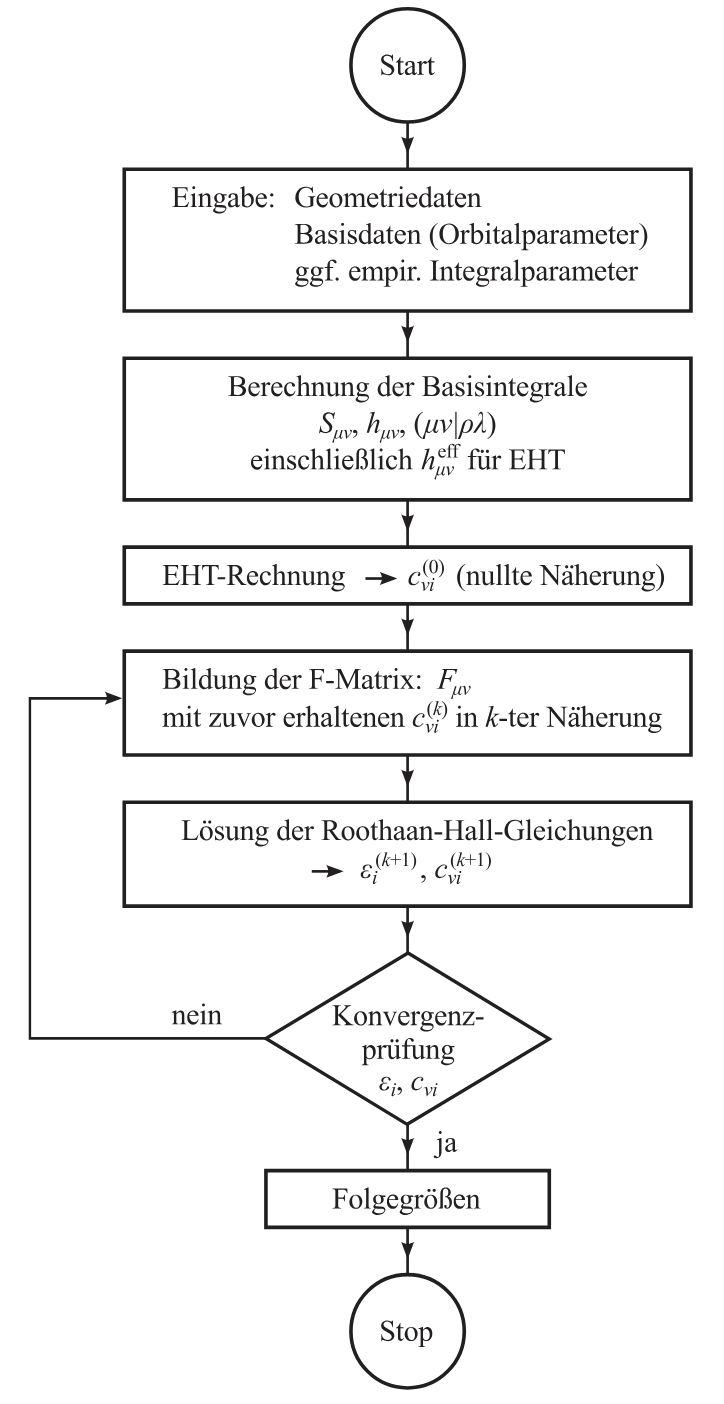
\includegraphics[width=.2\textwidth]{Graphik/SCF.png}
    \caption{Eine graphische Darstellung der SCF Methode.\autocite{Zülicke2015}}
    \label{fig:scf}
\end{abbfigure}

% ========================
%  Listen in Latex
% ========================
\begin{itemize}
    \item \textbf{Orbitale vom Gaußschen Typ (GTOs)}: 
    \begin{equation}
        \chi_\mu(\mathbf{r}) = N x^{l} y^{m} z^{n} e^{-\alpha \|\mathbf{r} - \mathbf{R}\|^2}
    \end{equation}
    \begin{tabular}{@{}ll@{}}
        \( N \): & Normierungskonstante \\
        \( \alpha \): & Exponent (radialer Zerfall) \\
        \( (l, m, n) \): & Drehimpulsquantenzahlen \\
        \( \mathbf{R} \): & Kernkoordinate \((X, Y, Z)\)
    \end{tabular}
    \autocite{Reinhold2015}

    \item \textbf{Slater-Type Orbitals (STOs)}: 
    \[ e^{-\zeta \|\mathbf{r} - \mathbf{R}\|} \]
    \begin{itemize}
        \item[+] Bessere Approximation der Atomorbitale
        \item[-] Rechenintensive Integralberechnung
        \item[→] Nur für spezielle Anwendungen/Referenzrechnungen
    \end{itemize}
    \autocite{Reinhold2015,Zülicke2015,alma990015422030206446}
\end{itemize}

% ========================
%  TABELLEN
% ========================
% Externe Tabellendateien einbinden
Auf diese kann man wie Abbildungen verweisen: \textbf{\cref{tab:geometrie}}

\begin{table}[H]
    \centering
    \caption{Die gemessenen Winkel und Abstände der optimierten Geometrien. Die farbigen Atome zeigen die zwischen denen die jeweilige Größe gemessenen wurde. Die blauen Atome sind von dem 2,5-Dioxo-2,5-dihydrofuran-3-carbonitril und die grünen sind von dem 2,3-Dichlorcyclopenta-1,3-dien.}
    \label{tab:geometrie}
    \resizebox{\textwidth}{!}{%
    \begin{tabular}{@{}l S[table-format=3.3] S[table-format=3.3] S[table-format=1.3] S[table-format=1.3]@{}}
    \toprule
                     & {Diederwinkel / \si{\degree}}        & {Winkel / \si{\degree}}     & \multicolumn{2}{c}{intramolekulare Distanz / \si{\angstrom}} \\ \midrule
                     & {\ch{O=}{\color[HTML]{0099FF}C}\ch{-}{\color[HTML]{0099FF}C}(CN)\ch{-}{\color[HTML]{0099FF}C}H\ch{-}{\color[HTML]{0099FF}C}\ch{=O}} 
                     & {H{\color[HTML]{00CC66}C}\ch{-}{\color[HTML]{00CC66}C}H\textsubscript{2}\ch{-}{\color[HTML]{00CC66}C}H} 
                     & {NC\ch{-}{\color[HTML]{0099FF}C}\ch{-}{\color[HTML]{00CC66}C}H}        
                     & {H{\color[HTML]{0099FF}C}\ch{-}{\color[HTML]{00CC66}C}H}               \\
    Präkomplex       & 179.635                            & 103.941                   & 3.171                          & 3.159                         \\
    Übergangszustand & 175.785                            & 99.973                    & 2.309                          & 2.038                         \\
    Produkt          & 177.903                            & 93.887                    & 1.590                          & 1.570                         \\ 
    \bottomrule
    \end{tabular}%
    }
\end{table}
\begin{table}[H]
    \caption{Die berechneten Energiedifferenzen in \unit{\kilo\joule\per\mole}.}
    \centering
    \begin{threeparttable}
    \label{tab:energie}
    \begin{tabular}{@{}l *{4}{S[table-format=-3.2]} @{}}
    \toprule
                                  & {DFT}         & {DFT + ZPE}    & {CC}          & {CC + ZPE}     \\
                                  & \multicolumn{4}{|c|}{\unit{\kilo\joule\per\mol}} \\ \midrule
    \makecell{Edukte - Präkomplex \\ (\textbf{Assoziationsenergie})}          &  -37.24        &  -34.02         &  -32.39        &  -29.17         \\
    \makecell{Edukte - Übergangszustand \\ (\textbf{Aktivierungsenergie})} & 16.40        & 23.07         & 20.78        & 27.45         \\
    \makecell{Edukte - Produkt \\ (\textbf{thermodynamische Energie}\textsuperscript{a})}             &  -90.75        &  -72.57         & -135.71        & -117.52         \\
    \bottomrule
    \end{tabular}
    
    \begin{tablenotes}
    \item[a] Auch als Reaktionsenthalpie \textDelta H bekannt, wird aber im weiteren Verlauf mit \textDelta E bezeichnet
    \end{tablenotes}
    \end{threeparttable}
\end{table}

\newpage

\section[Methoden und Modelle]{Methoden und Modelle}



\newpage

\section[Auswertung]{Auswertung}



\newpage

\section[Auswertung]{Auswertung}


\newpage

\section[Fehlerrechnung]{Fehlerrechnung}


\newpage

\section[Anhang]{Anhang}


\newpage

\section{Literaturverzeichnis}
\printbibliography[heading=none]

\end{document}
